\subsection{Architecture of proposed work}

\begin{frame}{Thesis Proposal}{Architecture of proposed work}
	
	\begin{minipage}[t]{0.48\linewidth}
\vspace{-2em}
		\begin{figure}[ht!]
			\centering
			\includegraphics[width=0.4\textwidth,keepaspectratio]{figures/40.Method/pyramid}
			\caption{Overall functional architecture of a smart metering system.}
		\end{figure}

	\end{minipage}\hfill
\pause
	\begin{minipage}[t]{0.48\linewidth}
		
		\vspace{2em}
		\begin{figure}[ht!]
			\centering

			\includegraphics[width=\textwidth,keepaspectratio]{figures/40.Method/data_flow}
			\caption{Data flow of measurement-information layers.}
		\end{figure}
	\end{minipage}
\pause
\begin{block}{\textbf{Architecture of proposed work}}
	
		\begin{enumerate}
		\item  Energy metering node:\\Non-intrusive self-powered sensor node;
		\item  Data transmission \&  Storage System: \\RTS wireless network
	\end{enumerate}
		
	
		

	
\end{block}

\end{frame}

%%%%%%%%%%%%%%%%%%%%%%%%%%%%%%%%%%%%%%%%%%%%%%%%%%%%%%%%%%%%%%%%%%%%%%%%%%%%%%%%%%%%%

%\begin{frame}{Thesis Proposal}{Architecture of proposed work}

%	\begin{figure}[ht!]
%		\centering
%		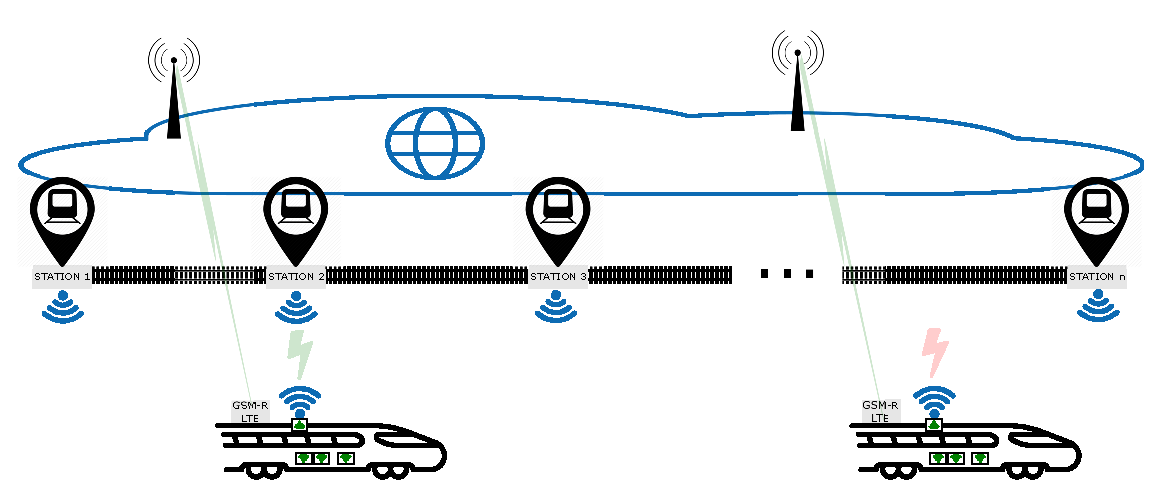
\includegraphics[width=0.9\textwidth,keepaspectratio]{figures/40.Method/architecture}
%		\caption{Architecture of proposed work.}
%	\end{figure}
		

%\end{frame}
%%%%%%%%%%%%%%%%%%%%%%%%%%%%%%%%%%%%%%%%%%%%%%%%%%%%%%%%%%%%%%%%%%%%%%%%%%%%%%%%%%%%%


\subsection{Part 1 --- Energy metering node}


\begin{frame}{Thesis Proposal}{Energy metering node}
\begin{block}{\textbf{Part 1 --- Energy metering node: \\ \small{Non-intrusive self-powered sensor node}}}
	\begin{figure}[ht!]
		\centering
		\includegraphics[width=0.45\textwidth,keepaspectratio]{figures/40.Method/powerSensing}
		\caption{Power architecture of case-study train.}
	\end{figure}
\end{block}
\end{frame}
%%%%%%%%%%%%%%%%%%%%%%%%%%%%%%%%%%%%%%%%%%%%%%%%%%%%%%%%%%%%%%%%%%%%%%%%%%%%%%%%%%%%%

\begin{frame}{Thesis Proposal}{Energy metering node}
\begin{block}{\textbf{Energy metering node --- Methodology}}

	\begin{figure}[ht!]
		\centering
		\includegraphics[width=0.75\textwidth,keepaspectratio]{figures/40.Method/methodElectrical}
		\caption{Models needed for simulation. Energy measurement system.}
	\end{figure}

\end{block}
\end{frame}
%%%%%%%%%%%%%%%%%%%%%%%%%%%%%%%%%%%%%%%%%%%%%%%%%%%%%%%%%%%%%%%%%%%%%%%%%%%%%%%%%%%%%

\begin{frame}{Thesis Proposal}{Energy metering node}
\begin{block}{\textbf{Energy metering node --- Contributions}}
		\begin{itemize}
			\item \textbf{New energy metering architecture}, according to some specifications such as the usage of a non-intrusive approach.
			This architecture will generate energy information about the power flow of the railway system.
\pause			
			\item \textbf{Accurate estimation of power flow} into catenary, based on on-board measurements. The available parameters will be: (1) the RMS voltage, current and apparent power, (2) the instantaneous active power, reactive power, power factor and frequency, and (3) the cumulative energy consumptions in terms of kVAh, kVARh and KWh.
		\end{itemize}
\end{block}
\end{frame}


\subsection{Part 2 --- Data transmission \& Storage System}


\begin{frame}{Thesis Proposal}{Data transmission \& Storage System}
\begin{block}{\textbf{Part 2 --- Data transmission \& Storage System: \\ \small{RTS wireless network}}}
\begin{figure}[ht!]
	\centering
	\includegraphics[width=0.8\textwidth,keepaspectratio]{figures/40.Method/arch2}
	\caption{Data transmission \& Storage System.}
\end{figure}
\end{block}
\end{frame}
%%%%%%%%%%%%%%%%%%%%%%%%%%%%%%%%%%%%%%%%%%%%%%%%%%%%%%%%%%%%%%%%%%%%%%%%%%%%%%%%%%%%%

\begin{frame}{Thesis Proposal}{Data transmission \& Storage System}
\begin{block}{\textbf{RTS wireless network --- Methodology}}

\begin{figure}[ht!]
	\centering
	\includegraphics[width=0.8\textwidth,keepaspectratio]{figures/40.Method/methodWireless}
	\caption{Models needed for simulation - RTS Wireless Network.}
\end{figure}

\end{block}
\end{frame}
%%%%%%%%%%%%%%%%%%%%%%%%%%%%%%%%%%%%%%%%%%%%%%%%%%%%%%%%%%%%%%%%%%%%%%%%%%%%%%%%%%%%%

\begin{frame}{Thesis Proposal}{Data transmission \& Storage System}
\begin{block}{\textbf{RTS wireless network --- Contributions}}
\begin{itemize}
\item \textbf{Availability of measured data} from trains where currently limited/inexistent energy measurement is performed.

\pause
\item Data-rate increase of energy measurements, which will result on direct \textbf{increase on the quality of information of energy}. This increase will overcome the 5-minute data-rate that currently are used in energy meters.

\pause
\item A further contribution can be the reduction of the dependence of broadband real-time/continuous communication (such as \ac{LTE}), with the direct cost reduction of information transmission of energy \ac{RTS} data.
\end{itemize}
\end{block}
\end{frame}

%%%%%%%%%%%%%%%%%%%%%%%%%%%%%%%%%%%%%%%%%%%%%%%%%%%%%%%%%%%%%%%%%%%%%%%%%%%%%%%%%%%%%
\subsection{Thesis Work Plan}
%%%%%%%%%%%%%%%%%%%%%%%%%%%%%%%%%%%%%%%%%%%%%%%%%%%%%%%%%%%%%%%%%%%%%%%%%%%%%%%%%%%%%

\begin{frame}{Thesis Proposal}{Work Plan}
\begin{figure}[ht!]
	\centering
	\includegraphics[width=0.7\textwidth,keepaspectratio]{figures/40.Method/workplan0}
	\caption{PhD Work Plan.}
\end{figure}
\end{frame}
%%%%%%%%%%%%%%%%%%%%%%%%%%%%%%%%%%%%%%%%%%%%%%%%%%%%%%%%%%%%%%%%%%%%%%%%%%%%%%%%%%%%%
